\documentclass[10pt]{article}
\usepackage[utf8]{inputenc}
\usepackage[doublespacing]{setspace}
\usepackage{textcomp}
\usepackage{amsmath,amssymb,amsthm}
\usepackage{fancyhdr}
\usepackage{lastpage}
\usepackage[]{hyperref}
\usepackage[pdftex]{graphicx}
\usepackage{ctex}
\usepackage{booktabs}
\usepackage{subfigure}
\usepackage{titlesec}
\usepackage{listings}
\usepackage{enumerate}
\usepackage{bm}
\usepackage{float}
\usepackage{url}
%\allowdisplaybreaks
\renewcommand{\contentsname}{\centerline{Contents}}
\pagestyle{fancy}
\author{D}
\def\name{D}
\lhead{Time Series Methods}
\chead{}
\rhead{\name}
\cfoot{-\space\thepage\space-}
\newtheorem{exer}{\bm{$Exercise$}}
\newtheorem{prob}{\bm{$Problem$}}
\newtheorem{bonus}{\bm{$Bonus\;Problem$}}
\newcommand{\tabincell}[2]{\begin{tabular}{@{}#1@{}}#2\end{tabular}}
\CTEXoptions[today=old]

\begin{document}

\title{Postgraduate Assignment}
\date{\today}
\maketitle
\thispagestyle{fancy}
\thispagestyle{fancy}

\begin{prob}
\end{prob}
\begin{enumerate}[1)]
\vspace{3mm}

\item
The formula for the Hodrick-Prescott (HP) filter is
\begin{align*}
&y_t=\tau_t+c_t,\\
&\min_{\tau_t, c_t}\{\sum^T_{t=1}(y_t-\tau_t)^2+\lambda\sum^{T-1}_{t=2}[(\tau_{t+1}-\tau_t)-(\tau_t-\tau_{t-1})]^2\},\\
&\textrm{or},\;\min_{\tau_t, c_t}\{\sum^T_{t=1}c_t^2+\lambda\sum^{T-1}_{t=2}[(\tau_{t+1}-\tau_t)-(\tau_t-\tau_{t-1})]^2\}.
\end{align*}
Explanations:\\
$t$ - the time\\
$y_t$ - the original time series\\
$\tau_t$ - the trend component of the time series\\
$c_t$ - the cyclical component of the time series\\
$T$ - the maximized or end time\\
$\lambda$ - the penalty parameter, the greater it is the smoother the resulting trend will be\footnote{ Falk, B. (2006). \textit{Lecture 21 - modeling and estimating trends: III}. Retrieved from \url{http://www2.econ.iastate.edu/classes/econ674/falk/lecture_21_trends_III.pdf}}
\vspace{3mm}

\item
The HP filter minimizes the two terms, $\sum^T_{t=1}c_t^2$ and $\lambda\sum^{T-1}_{t=2}[(\tau_{t+1}-\tau_t)-(\tau_t-\tau_{t-1})]^2$.\\
What each of the two terms does:\\
$\sum^T_{t=1}c_t^2$ - the sum of the squared deviation of $y_t$ from the trend, penalizing the variance of $c_t$\\ % Comment: variance is $\frac{1}{n-1}\sum{(c_t-\tau_t)^2}$
$\lambda\sum^{T-1}_{t=2}[(\tau_{t+1}-\tau_t)-(\tau_t-\tau_{t-1})]^2$ - the sum of the squared second differences in the trend, penalizing the changes in the trends's growth rate, or called the lack of smoothness in $\tau_t$\\
How the two terms play together:\\
The connection is $y_t=\tau_t+c_t$. ``The HP filter identifies the cyclical component $c_t$ from $y_t$ by the trade-off to the extent to which the trend component keeps track of the original series $y_t$ (good fit) against the prescribed smoothness in $\tau_t$.''\footnote{ Kim, H. (2004). \textit{Hodrick-Prescott filter}. Retrieved from \url{http://webhome.auburn.edu/~hzk0001/hpfilter.pdf}.}
\vspace{3mm}

\item
The second-order difference is the discrete analogy to the second-derivative. For a discrete time series, the second-order difference represents the curvature of the series at a given time point. The curvature, namely the lack of smoothness, is what the HP filter tries to minimize. The second-order difference in this case is
\begin{align*}
\Delta^2\tau_{t+1}&=\Delta(\Delta\tau_{t+1})\\
&=\Delta(\tau_{t+1}-\tau_{t})\\
&=\Delta\tau_{t+1}-\Delta\tau_{t}\\
&=(\tau_{t+1}-\tau_t)-(\tau_t-\tau_{t-1})\\
&=\tau_{t+1}-2\tau_t+\tau_{t-1}
\end{align*}
$\Delta^2\tau_{t+1}$ is positive if $\Delta\tau_{t+1}>\Delta\tau_{t}$ and negative if $\Delta\tau_{t+1}<\Delta\tau_{t}$. If there is more upward (less downward) change in the time series at a time point than in the previous time point, there is positive curvature; else, there is a negative curvature.\footnote{ Ben (https://stats.stackexchange.com/users/173082/ben). (2018) \textit{What is the intuition behind second order differencing?} Retrieved from \url{https://stats.stackexchange.com/q/351753}}. % Comment: This puts no penalty on a linear trend. Hence, the estimate tends to be a linear trend.
\vspace{3mm}

\item
$\lambda$ is the pre-specified parameter and controls the smoothness of the trend $\tau_t$.\\
How changing $\lambda$ affects the output:
\begin{align*}
&\tau_t\rightarrow\textrm{linear trend},\;\textrm{as}\;\lambda\rightarrow\infty,\\
&\tau_t\rightarrow{y_t}\;\textrm{and}\;c_t=0,\;\textrm{as}\;\lambda\rightarrow0.
\end{align*}
In other words, if $\lambda=0$, then $c_t=0$ and $\tau_t=y_t$, as $t=1,2,...,T$; if $\lambda\rightarrow\infty$, then $\tau_t$ is the linear trend obtained by fitting $y_t$ to a linear trend model by OLS.\\
How this parameter can be choose:\\
In practice, Hodrick and Prescott suggest that $\lambda=1600$ is a reasonable choice for quarterly data, $\lambda\in(100000,150000)$ is for monthly data, and $\lambda\in(5,15)$ is for annual data.\footnote{ Gulan, Adam. (2019). \textit{Macroeconomics theory; lectures 1 and 2}. Retrieved from \url{http://www.gulan.pl/lectures1-2.pdf}}\footnote{ Falk, B. (2006). \textit{Lecture 21 - modeling and estimating trends: III}. Retrieved from \url{http://www2.econ.iastate.edu/classes/econ674/falk/lecture_21_trends_III.pdf}}
\vspace{3mm}

\item
One answer:\\
The use of the HP filter requires the minimizer explicitly to be computed. A relatively simple minimization method in practice is to calculate the mean squared error (MSE), which is a measure of the quality of an estimator,
\begin{align*}
MSE=\frac{1}{n}\sum_{i=1}^{n}(Y_i-\hat{Y}_i)^2. % Comment: This does not produce $\tau_t$.
\end{align*}
Name another statistical method that is estimated with the minimization method:\\
The least squares fitting, which finds the best-fitting curve to a given set of points by minimizing the sum of the squares of the offsets of the points from the curve, is estimated with the same method.\footnote{ Weisstein, E. W. (n.d.). \textit{Least squares fitting}. Retrieved from \url{http://mathworld.wolfram.com/LeastSquaresFitting.html}}
% Comment: But how does WH compute \tau_t. We have to solve a least squares problem like OLS for linear regression.

Another answer:\\
The HP filter is a special case of the Whittaker-Henderson (WH) method of graduation or smoothing, which is frequently used in the actuarial literature.\\
Name another statistical method that is estimated with the WH method:\\
The method of P-splines, with the equation $\hat{\mu}=(B'B+\lambda{D'}D^{-1}B'y)$, evolved from the Whittaker smoothing $\hat{\mu}=(I+\lambda{D'}D)^{-1}$, where $B$ is a regression matrix of B-splines of degree $d$ and $B=I$ is a special case and hence the Whittaker smoothing
\footnote{ Yamada, H. (2018). Why does the trend extracted by the Hodrick-Prescott filtering seem to be more plausible than the linear trend? \textit{Applied Economics Letters}, 25(2), 102-105. Retrieved from \url{https://doi-org.ezproxy.canterbury.ac.nz/10.1080/13504851.2017.1299095}.}\footnote{ Currie, I. (2019). \textit{Back to the future with Whittaker smoothing}. Retrieved from \url{https://www.longevitas.co.uk/site/informationmatrix/whittaker.html}.}
\vspace{3mm}

\item
The suitable data chosen from the previous three assignments:\\
Signal in Noise (Problem 3, Assignment One)
\begin{figure}[H]
  \centering
  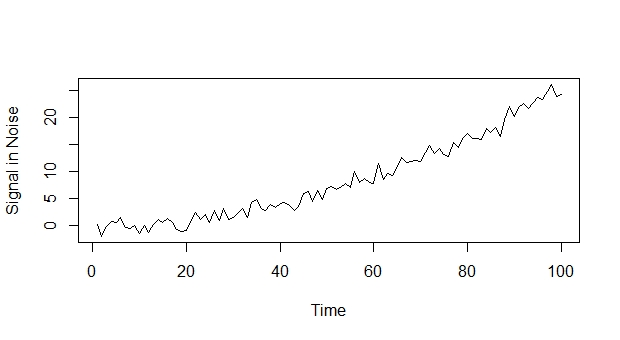
\includegraphics[width=10cm,height=5cm]{p16a.jpeg}
  \caption{Signal time series} % Comment: This is not real data.
\end{figure}
Closing Price of the SP500 (Problem 4, Assignment One)
\begin{figure}[H]
  \centering
  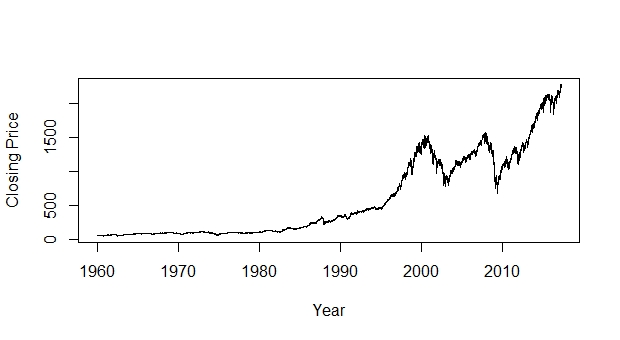
\includegraphics[width=10cm,height=5cm]{p16b.jpeg}
  \caption{Price time series}
\end{figure}
NZ Unemployment Rates (Problem 4, Assignment Two)
\begin{figure}[H]
  \centering
  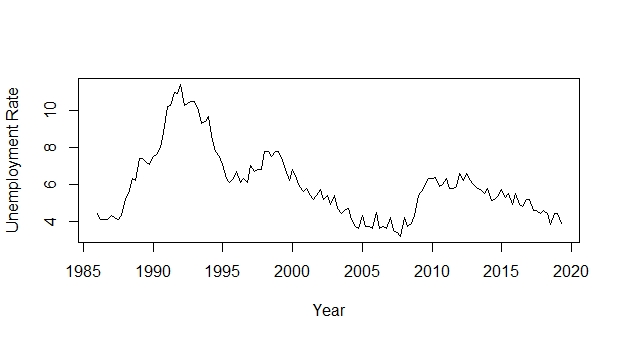
\includegraphics[width=10cm,height=5cm]{p16c.jpeg}
  \caption{Unemployment rate time series}
\end{figure}
Reasons:\\ % Comment: SP500 has no annual features, only 5-10 years business cycles.
Short-term fluctuations can be found in the three cases above, and the latter two cases have clearly quarterly or annual features. In practice, the HP filter is commonly applied to remove these short-term fluctuations and reveal the long-term trends, and in Problem 4 we know suggested $\lambda$ for quarterly and annual data. Therefore, I selected these three cases for such purposes.\footnote{ Kenton, W. (2019). \textit{Hodrick-Prescott (HP) filter}. Retrieved from \url{https://www.investopedia.com/terms/h/hpfilter.asp}.}
\vspace{3mm}

\item
We will simply run the HP filter on the three cases and perform more in details on the third case. With the library ``mFilter'', the trend line and the cyclical component are revealed respectively.\\
Case 1:\\
R codes:
\lstinputlisting{p17a.R}
R outputs:
\begin{figure}[H]
  \centering
  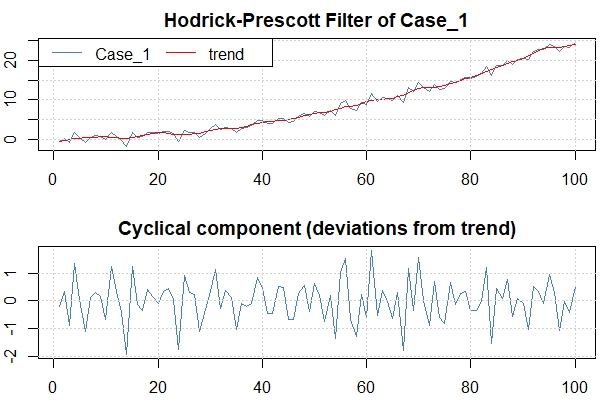
\includegraphics[width=10cm,height=7.5cm]{p17a.jpeg}
  \caption{Apply the HP filter to the signal in noise}
\end{figure}
Case 2:\\
R codes:
\lstinputlisting{p17b.R}
R outputs:
\begin{figure}[H]
  \centering
  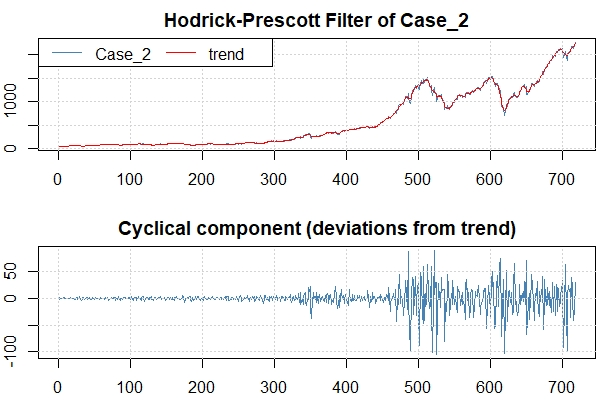
\includegraphics[width=10cm,height=7.5cm]{p17b.jpeg}
  \caption{Apply the HP filter to the closing Price of the SP500}
\end{figure}
Case 3:\\
R codes:
\lstinputlisting{p17c.R}
R outputs:
\begin{figure}[H]
  \centering
  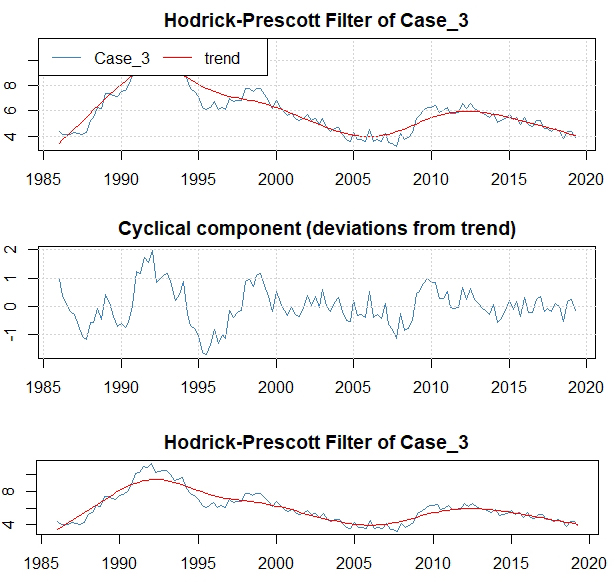
\includegraphics[width=10cm,height=10.5cm]{p17c.jpeg}
  \caption{Apply the HP filter to the NZ unemployment rate, with and without legends and grids}
\end{figure}
More on Case 3:\\
R codes:
\lstinputlisting{p17d.R}
R outputs:
\begin{figure}[H]
  \centering
  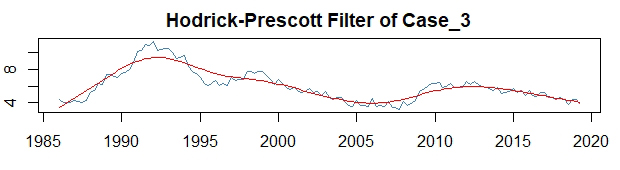
\includegraphics[width=10cm,height=3cm]{p17d.jpeg}
  \caption{Apply the HP filter with $\lambda=1600$}
\end{figure}
\begin{figure}[H]
  \centering
  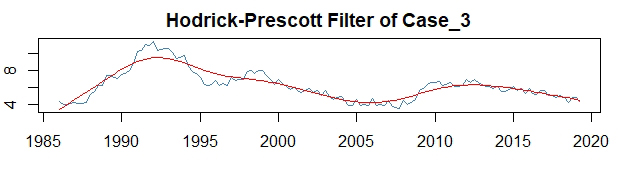
\includegraphics[width=10cm,height=3cm]{p17e.jpeg}
  \caption{Apply the HP filter with $\lambda=1600$ and the drift}
\end{figure}
\begin{figure}[H]
  \centering
  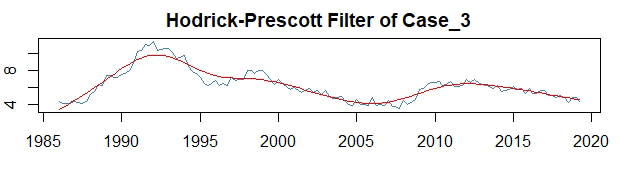
\includegraphics[width=10cm,height=3cm]{p17f.jpeg}
  \caption{Apply the HP filter with $\lambda=800$ and the drift}
\end{figure}
\begin{figure}[H]
  \centering
  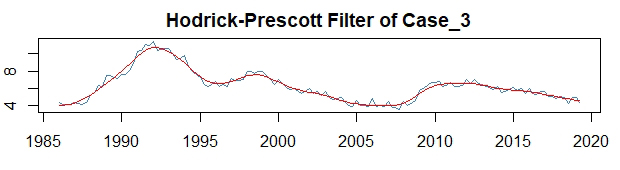
\includegraphics[width=10cm,height=3cm]{p17g.jpeg}
  \caption{Apply the HP filter with $\lambda=52$ and the drift}
\end{figure}
\begin{figure}[H]
  \centering
  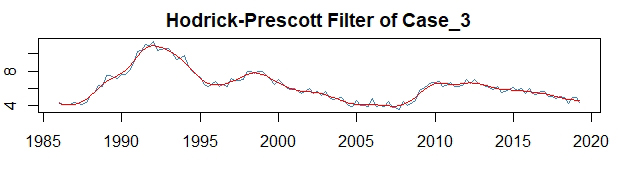
\includegraphics[width=10cm,height=3cm]{p17h.jpeg}
  \caption{Apply the HP filter with $\lambda=12$ and the drift}
\end{figure}
\begin{figure}[H]
  \centering
  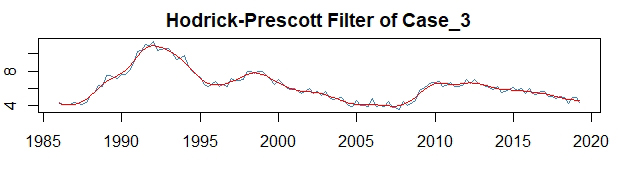
\includegraphics[width=10cm,height=3cm]{p17i.jpeg}
  \caption{Apply the HP filter with $\lambda=15$ and the drift}
\end{figure}
\begin{figure}[H]
  \centering
  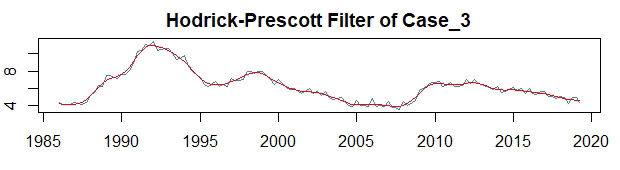
\includegraphics[width=10cm,height=3cm]{p17j.jpeg}
  \caption{Apply the HP filter with $\lambda=6$ and the drift}
\end{figure}
\vspace{3mm}
The value chosen:\\
$\lambda=12$\\
Explanations:\\
Though $\lambda=1600$ is suggested in Problem 4, through my observation, when $\lambda=12$, $15$ or $6$ with the drift, the HP filter works well, because it not only makes the line smooth, with the unwanted short-term fluctuations removed, but also minimizes the difference between the filtered line and the original line, with the long-term fluctuations kept. There are few differences observed among $\lambda=12$, $15$ and $6$, so the median $12$ is selected.\\
Interpretations:\\
The importance of the short-term unemployment fluctuations has been discounted by the HP filter. We can clearly see the local maximized unemployment rates are around 1992, 1998 and 2012; the local minimized rates are around 1996 and 2008. The long-term trends of the NZ unemployment rates are upward between 1986 and 1992 and downward after 1992. This is the result I expect. However, one problem is that it looks all the short-term fluctuations are removed without distinction, including the ones around the maximums and the minimums that I want to see.

\end{enumerate}

\end{document}
